% Paste these two lines in the paper preamble if they are not already present:
% \usepackage{tikz}
% \usetikzlibrary{positioning}

\paragraph{Additional topology mutations.}
Beyond branch expansion and the conversion of parallel workers into a
serializer, the traces exhibit two additional forms of topology adaptation.
First, the system can rewire communication without changing the agent set.
In the PlanCraft trace \texttt{VAL0403/run\_2}, the auditor detected premature
consensus: all three agents agreed even though confidence was imperfect and
unresolved issues remained.  The repair replaced the coordinator-centered
star with a fully connected debate topology (Figure~\ref{fig:mutation-debate}).
The following turn contained no detected process failure, terminated by
consensus with confidence $1.0$, and received benchmark score $1.0$.

\begin{figure}[t]
  \centering
  \resizebox{\columnwidth}{!}{%
  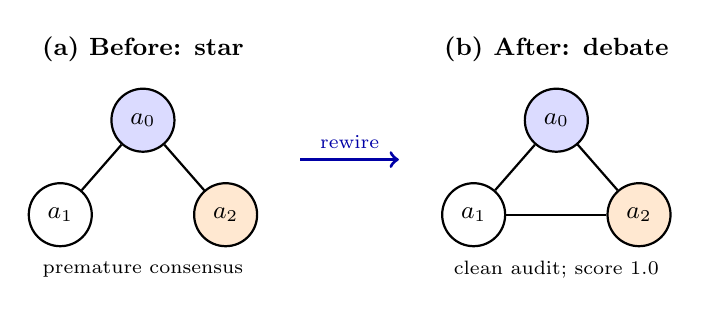
\begin{tikzpicture}[
      agent/.style={circle, draw, thick, minimum size=8mm, font=\small},
      coord/.style={agent, fill=blue!14},
      verify/.style={agent, fill=orange!18},
      link/.style={thick},
      mutation/.style={->, very thick, blue!65!black},
      panel/.style={font=\small\bfseries}
    ]
    % Before: star
    \node[panel] at (0,1.75) {(a) Before: star};
    \node[coord]  (s0) at (0,0.85) {$a_0$};
    \node[agent]  (s1) at (-1.05,-0.35) {$a_1$};
    \node[verify] (s2) at (1.05,-0.35) {$a_2$};
    \draw[link] (s0)--(s1);
    \draw[link] (s0)--(s2);
    \node[font=\scriptsize, align=center] at (0,-1.05)
      {premature consensus};

    % Mutation arrow
    \draw[mutation] (2.0,0.35)--(3.25,0.35)
      node[midway, above, font=\scriptsize, align=center]
      {rewire};

    % After: debate
    \node[panel] at (5.25,1.75) {(b) After: debate};
    \node[coord]  (d0) at (5.25,0.85) {$a_0$};
    \node[agent]  (d1) at (4.20,-0.35) {$a_1$};
    \node[verify] (d2) at (6.30,-0.35) {$a_2$};
    \draw[link] (d0)--(d1);
    \draw[link] (d0)--(d2);
    \draw[link] (d1)--(d2);
    \node[font=\scriptsize, align=center] at (5.25,-1.05)
      {clean audit; score $1.0$};
  \end{tikzpicture}%
  }
  \caption{Communication rewiring in PlanCraft
  \texttt{VAL0403/run\_2}. The mutation preserves all three agents but replaces
  the coordinator-centered star with an all-to-all debate, adding the missing
  worker--verifier communication edge. Blue denotes the coordinator and orange
  the verifier.}
  \label{fig:mutation-debate}
\end{figure}

Second, the system can insert a role-specific validation stage rather than
expanding a failing branch with additional workers.  In Math500
\texttt{test\_geometry\_248/run\_1}, the initial singleton produced a
low-confidence answer with no downstream critic.  The repair added one agent
with structural role \emph{verifier} and stage role \emph{critic}, then changed
the group to a two-agent debate (Figure~\ref{fig:mutation-verifier}).  The next
audit was clean, the run terminated by consensus with confidence $1.0$, and the
answer received benchmark score $1.0$.  This is a role-conditioned node
insertion: the added computation is explicitly assigned to validation rather
than to another independent solution branch.

\begin{figure}[t]
  \centering
  \resizebox{\columnwidth}{!}{%
  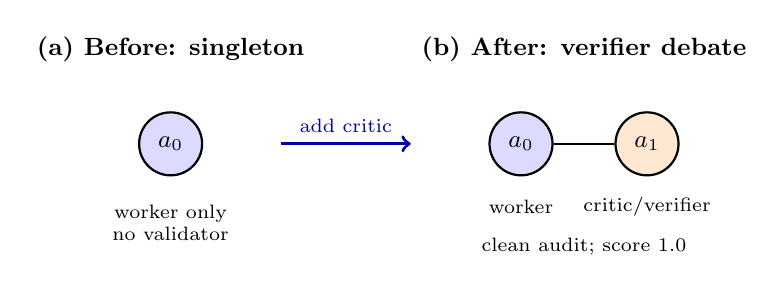
\begin{tikzpicture}[
      agent/.style={circle, draw, thick, minimum size=8mm, font=\small},
      worker/.style={agent, fill=blue!14},
      verify/.style={agent, fill=orange!18},
      link/.style={thick},
      mutation/.style={->, very thick, blue!65!black},
      panel/.style={font=\small\bfseries}
    ]
    % Before: singleton
    \node[panel] at (0,1.45) {(a) Before: singleton};
    \node[worker] (w0) at (0,0.25) {$a_0$};
    \node[font=\scriptsize, align=center] at (0,-0.75)
      {worker only\\no validator};

    % Mutation arrow
    \draw[mutation] (1.40,0.25)--(3.05,0.25)
      node[midway, above, font=\scriptsize, align=center]
      {add critic};

    % After: worker-verifier debate
    \node[panel] at (5.25,1.45) {(b) After: verifier debate};
    \node[worker] (w1) at (4.45,0.25) {$a_0$};
    \node[verify] (v1) at (6.05,0.25) {$a_1$};
    \draw[link] (w1)--(v1);
    \node[font=\scriptsize] at (4.45,-0.55) {worker};
    \node[font=\scriptsize] at (6.05,-0.55) {critic/verifier};
    \node[font=\scriptsize, align=center] at (5.25,-1.05)
      {clean audit; score $1.0$};
  \end{tikzpicture}%
  }
  \caption{Role-conditioned node insertion in Math500
  \texttt{test\_geometry\_248/run\_1}. A missing-validator signal changes a
  singleton into a worker--verifier debate. The mutation increases the agent
  count by one while assigning the new node a distinct validation role.}
  \label{fig:mutation-verifier}
\end{figure}

Together with branch expansion and serialization, these examples expose four
qualitatively different adaptation mechanisms: growing a local subgroup,
serializing execution, rewiring communication among existing agents, and
inserting a specialized validation role.
